%-------------------------------------------------------------------------------
% seq64_meta_events
%-------------------------------------------------------------------------------
%
% \file        seq64_meta_events.tex
% \library     Documents
% \author      Chris Ahlstrom
% \date        2017-07-23
% \update      2017-08-13
% \version     $Revision$
% \license     $XPC_GPL_LICENSE$
%
%     Provides a discussion of the MIDI GUI meta_events that Sequencer64
%     supports.
%
%-------------------------------------------------------------------------------

\section{Sequencer64 Meta Event / SysEx Support}
\label{sec:meta_events}

   In recent versions of \textsl{Sequencer64} we are attempting better support
   for MIDI Meta and System Exclusive events, as well as a Tempo track.
   At present (v. 0.93+), \textsl{Sequencer64} now supports the display of Set
   Tempo and Time Signature events.  They can also be added and edited, in
   various ways.  For example, see \sectionref{sec:seq64_event_editor}.
   Only the first Time Signature event is used to modify playback.
   System Exclusive support is also still in progress.

   This section consolidates the description of the meta-event support.
   The following topics apply:

   \begin{enumerate}
      \item Tempo display min/max in "usr" settings.
      \item Tempo display in main window.
      \item Tempo display in pattern editor.
      \item Tempo display in song editor.
      \item Tempo and Time signature display and editing in the event editor.
   \end{enumerate}

   Before we discuss these items, we need to note \textsl{how} the tempo track is
   implemented in \textsl{Sequencer64}.  Rather man make a SeqSpec track for
   the tempo events, we follow the MIDI specification, which mandates that
   Tempo events must occur only in the first track.  \textsl{Sequencer64} has
   been upgraded so that Set Tempo and Time Signature events are full-fledged
   MIDI events and can be viewed (and later, edited) in the existing
   user-interface elements.  Notes and other events can occur in the same
   track, if the user-musician so desires.

   To reiterate, track 1 (pattern 0) is the only track where tempo events
   can be placed and edited.

\subsection{"usr" BPM Display Settings}
\label{subsec:meta_events_usr}

   \textsl{Sequencer64} allows the tempo to range from 1 to 600 BPM
   (beats per minute).
   This range is hardwired into the application.
   But we need to be able to display tempo with a little more granularity.
   Therefore, \textsl{Sequencer64} provides some scaling for the tempo
   displays.  These values are found in the "usr" file:

   \begin{verbatim}
		0         # midi_bpm_minimum
		360       # midi_bpm_maximum
   \end{verbatim}

   See \sectionref{subsec:seq64_usr_file_user_midi_settings}, for more
   information.  This setting can only be made by editing the "usr" file
   while \textsl{Sequencer64} is not running.
   Note that this setting affects the global BPM setting ("c\_bpmtag").

% DO THESE SETTINGS apply to the global BPM or the tempo-track BPM???

\subsection{Composite Display of Tempos}
\label{subsec:meta_events_composite_display}

The following figure shows a composite picture of the various representations
of Set Tempo events.

\begin{figure}[H]
   \centering 
   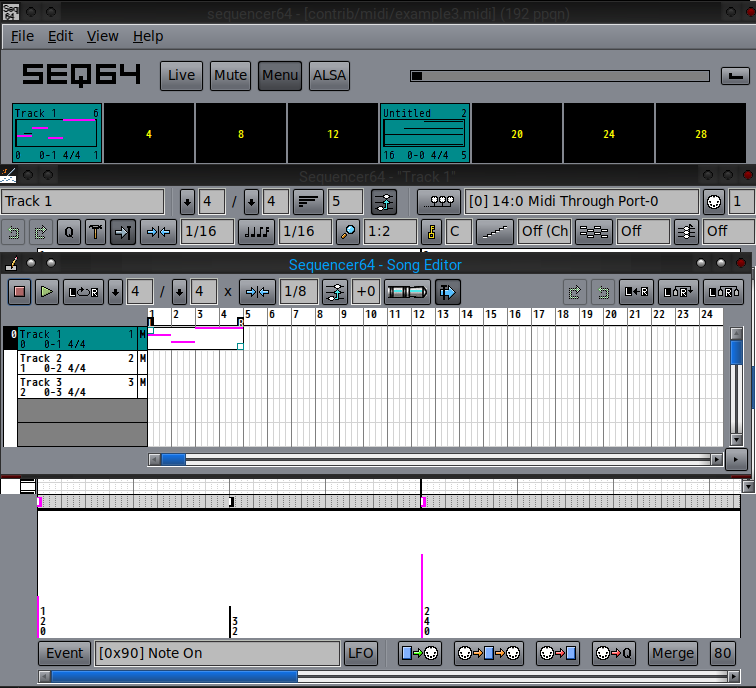
\includegraphics[scale=0.75]{meta/combined_tempo_display.png}
   \caption{Various Tempo Displays}
   \label{fig:meta_events_tempo_displays}
\end{figure}

The top of the figure shows the magenta tempo lines in a pattern slot that
is currently being edited.  This view cannot be directly edited, but the event
editor and the main window's BPM settings can be used to add, delete, or adjust
the tempo.

The middle shows the very similar representation of the tempo in the Song
Editor.  Again, this view does not (currently) allow editing of the tempo
events.

The bottom shows tempo as an event (in the event strip) and a data value
in the data pane.  A tempo event can be added here by holding the Ctrl key
and painting an event in the event strip, and it can then be modified by
same method that note velocities can be edited.  Note that tempo events 
are \textsl{always} shown in the event strip and the data pane, no matter
what other \textbf{Event} type has been selected.

\subsection{Tempo in the Main Window}
\label{subsec:meta_events_mainwid}

% The following figure shows a note and some tempo changes.
%
% \begin{figure}[H]
%   \centering 
%   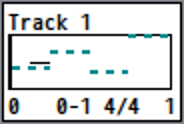
\includegraphics[scale=1.0]{meta/mainwid_pattern_tempo.png}
%   \caption{Tempo in Pattern Slot}
%   \label{fig:meta_events_mainwid_slot}
% \end{figure}
%
% This figure is out-of-date.

The tempo is shown as a solid magenta-colored line at the relative height
for the tempo,
based on the minimum and maximum values configured in the "usr" file as
discussed in the previous section.
This pattern-slot tempo display is rudimentary.  It doesn't allow for ramping
of the tempo at present (except by recording while holding the BPM
spin-control), and cannot be directly edited in this window.
However, tempos can be logged or recorded via magenta-colored controls at the
bottom of the main window.

\begin{figure}[H]
   \centering 
   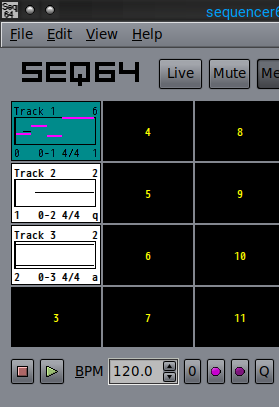
\includegraphics[scale=1.0]{meta/tempo_recording.png}
   \caption{Tempo Recording Controls}
   \label{fig:meta_events_mainwid_tempo_recording}
\end{figure}

The 0th pattern slot shown in the figure represents Track 1, the
MIDI Tempo track.  The magenta lines show the tempos already in that track.
Now look at the BPM control.  The first button to its right ("0") is the
tempo-tap button, used for setting a tempo by tapping in time to music.
The light-magenta button that comes next, when pressed while playback is
occurring, logs a tempo event at the current progress location and the
current BPM value in the BPM spin-field.  The dark magenta button to the right
of that toggles the mode of recording the changes to the BPM spin-button while
playback is occurring.  (The "Q" button is for keep-queues, and is unrelated to
tempo processing.)

Now, although track 1 (pattern 0) might start out with a length of only a
measure or two, the performance continually ticks upward, and tempo events that
are recorded after the end of the track at still recorded, and
\textsl{they will extend the length of the tempo track automatically}.
If the "show sequences key" option is enabled, the length of each track, in
measures, is shown at the top right of each main window pattern slot, so it can
be tracked by the user.

Once tempo events have been recorded, they can be tweaked (or deleted)
either in the pattern editor or in the event editor.  Generally, they are
treated like control events that are always available.  Deleting all tempo
events will not reduce the (possibly new) length of the sequence.

One more thing to note about the Tempo track is that it will
\textsl{not} change tempo unless that track is unmuted.
This behavior is a feature, not a bug.

% \subsubsection{MIDI Metrics, PPQN}
% \label{subsubsec:meta_events_midi_ppqn}

%-------------------------------------------------------------------------------
% vim: ts=3 sw=3 et ft=tex
%-------------------------------------------------------------------------------
